%
% General structure for the revdetua class:
%

\documentclass[...]{revdetua}
\usepackage{graphicx}
%
% Valid options are:
%
%   longpaper --------- \part and \tableofcontents defined
%   shortpaper -------- \part and \tableofcontents not defined (default)
%
%   english ----------- main language is English (default)
%   portugues --------- main language is Portuguese
%
%   draft ------------- draft version
%   final ------------- final version (default)
%
%   times ------------- use times (postscript) fonts for text
%
%   mirror ------------ prints a mirror image of the paper (with dvips)
%
%   visiblelabels ----- \SL, \SN, \SP, \EL, \EN, etc. defined
%   invisiblelabels --- \SL, \SN, \SP, \EL, \EN, etc. not defined (default)
%
% Note: the final version should use the times fonts
% Note: the really final version should also use the mirror option
%




\begin{document}

\Header{Volume}{19}{Novembro}{2020}{1}
% Note: the month must be in Portuguese

\title{Exhaustive search application for the max clique problem}
\author{Rodrigo Ferreira} % or \author{... \and ...}
\maketitle

\begin{resumo}% Note: in Portuguese
 Este artigo começa por contextualizar conceitos essenciais ao tema do problema, como o conceito de grafo, nós, arestas, subgrafo e clique. Passa então descrever o problema em questão. Depois de estabelecidas tais bases, explica o conceito de algoritmos de pesquisa de força bruta e em particular, pesquisa exaustiva. As suas características, vantagens, desvantagens, e como se encaixa no problema em questão, assim como uma avaliação dos resultados obtidos.
\end{resumo}

\begin{abstract}% Note: in English
  This paper starts out by contextualizing important concepts essential to the understanding of its theme, like graphs, nodes, edges, subgraphs and cliques. Afterwards, the problem at hand is described. When the basic concepts and the problem are explained, we move on to the topic of brute force search, and exhaustive search in particular. Its characteristics, advantages, disadvantages, how it fits into this theme, as well as an evaluation of its results.
\end{abstract}
\section{Introduction}
\subsection{Fundamental concepts}
We can’t discuss the max clique problem without first establishing some key concepts.
Graphs are structures composed of 2 sets, a set V, of nodes, and a set E of edges (we are always talking about undirected graphs in this paper).
Nodes, vertices, or points are the fundamental unit of which graphs are formed, in a graph diagram they are objects usually represented by a circle with a label.
Edges are pairs of nodes, representing a relation between them, in the case at hand (undirected graphs), (i,j) implies (j,i), this isn’t the case for arcs in directed graphs but we’re not using that structure here. In a graph diagram, edges are usually represented by a line uniting two nodes.
Subgraph…
complete subgraph
Clique
\subsection{The problem}
Now that the basic concepts relevant to the problem have been estabilished, we can move on to describing the problem itself./////
The maximum clique of a graph $G$ is a complete subgraph $G'$ such that no other complete subgraf in 
$G$ has cardinality higher than $\#G'$.
It's a simple description to a difficult problem, as the maximum clique problem is ...
\section{The approach}
\subsection{Brute force algorithms}
Brute force algorithms use a straightforward approach to solving problems taking advantage of a computers computing power, over that of a human being.
It is usually directly based on the problem statement and definitions of concepts involved [1]. 
\subsection{Exhaustive search}
Exhaustive search is a brute force approach to combinatorial problems.
It generates all candidate answers, and then checks each of them to confirm their validity, returning the best.
This approach, though simple and effective, as it can tackle most problems we can think of and usually requires a very simple implementation, is extremely inefficient, due to its blind "try everything" approach. And thus, it's only advised for very small instances of the problems it can solve, due to its fast growth (timewise)///

\section{The algorithm}
A quality in brute force, and more specifically, exhaustive search algorithms is that the code is very simple.
It only takes a small function, which will be briefly described, to get the maximum clique(s) from a set of nodes N and a set of edges M.
First, we notice that the maximum clique for a graph $G$ with $1<=N$ vertices must have a cardinality between $1$ and $\#N$, $1$ assuming there are no edges, and $\#N$ assuming $G$ is a complete graph, and thus, a clique.
When we become aware of this, we can make a cycle where we generate all combinations (could be permutations but it would be useless because we're using undirected graphs, i.e. $(i,j)=(j,i)$) of vertices with size $1$ to $N$.
When we get all these combinations, we go one by one, and test if indeed there exists an edge for every pair of vertices in said combination, if it does constitute a clique, we append it to a structure (dictionary where the key represents the cardinality of the solutions it maps to, and the value is a list of subgraphs with that cardinality) containing all solutions, and update another variable, $max$, to keep track of the cardinality of the best solution so far, otherwise we ignore it.
once the program has run its course for all combinations of size $1$ to $N$, we obtain the maximum cliques by accessing our dictionary with $max$ as key.
	
\subsection{Complexity}
It's easy to see, given the algorithm's description, that its complexity depends only on the size of the set of vertices. ///worst best and average all the same...
$$\sum_{i=1}^{n}{{n}\choose{i}}{{i}\choose{2}}=2^{(n-3)}(n-1)n$$
\subsection{Testing for bigger instances}
\subsubsection{Basic operation count}
As we are working with an algorithm with complexity ///(insert complexity), we expect the amount of basic operations executed (an instruction in the innermost loop) to increase exponentially///check as $N$ increases.
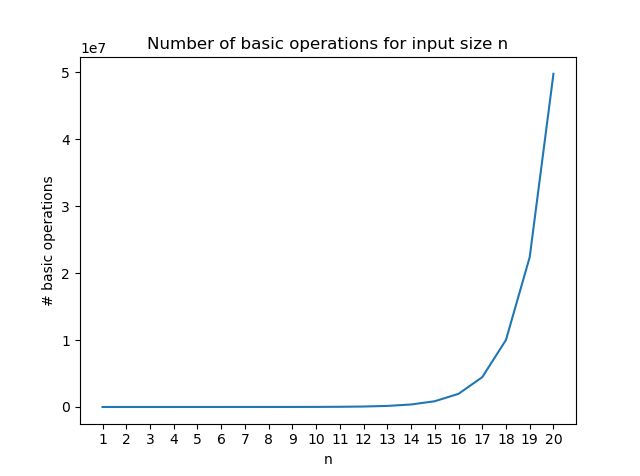
\includegraphics[scale=0.5]{basic_ops.png}
\subsubsection{Executing time}
As a consequence of the number of operations increasing by such a factor as $N$ grows, the executing time will increase very fast as well.
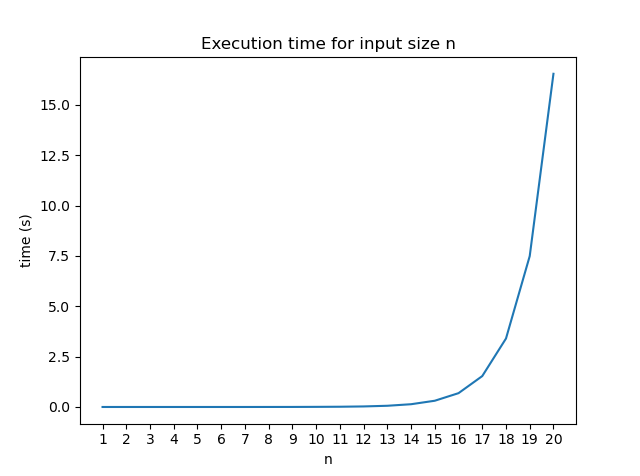
\includegraphics[scale=0.5]{exe_time.png}
\subsubsection{Solutions and total configurations}
On our formula it's clear the sheer amount of configurations generated for each $N$...
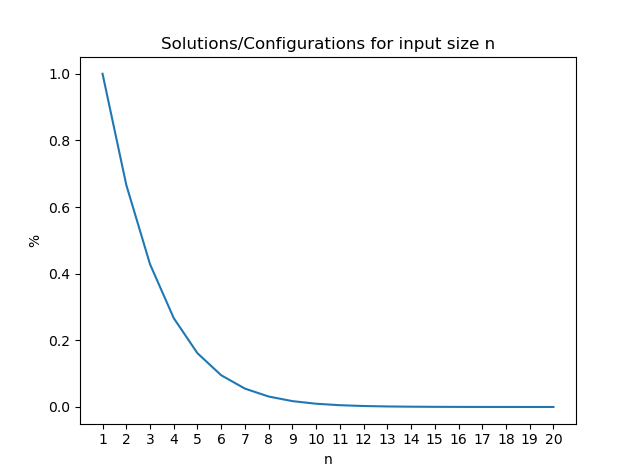
\includegraphics[scale=0.5]{solconfig.png}
\subsection{Comparing results}
The results seem to coincide with our previous complexity analysis...
\subsection{Estimating running time for bigger instances}
With our previous results we can pick an n, and get its number of operations and executing time,  $X=\frac{basic\ operations}{executing\ time}$ where $X$ gives us an estimate of the basic operations done per second, for a huge instance size $j$, we simply have to calculate its number of operations using our formula $$\sum_{i=1}^{n}{{n}\choose{i}}{{i}\choose{2}}=2^{(n-3)}(n-1)n$$
with $n=j$, we can then multiply that number of operations with $X$ to get an estimate of the running time for an instance of size $j$.

\section{Conclusions}
This example was effective at showing the pros and cons of exhaustive search algorithms, we managed to make a very simple program, that works very well for smaller instances of our problem, but scales very poorly, leaving us to wait for an answer, which might take an unimaginable amount of time and huge computational resources to achieve.

\bibliography{...} % use a field named url or \url{} for URLs
% Note: the \bibliographystyle is set automatically

\end{document}
